\documentclass[conference]{IEEEtran}
\usepackage{cite}
\usepackage{amsmath,amssymb,amsfonts}
\usepackage{algorithmic}
\usepackage{graphicx}
\usepackage{textcomp}
\usepackage{xcolor}
\usepackage{float}
\usepackage{booktabs}
\usepackage{url}
\usepackage{siunitx}

\def\BibTeX{{\rm B\kern-.05em{\sc i\kern-.025em b}\kern-.08em
    T\kern-.1667em\lower.7ex\hbox{E}\kern-.125emX}}

\begin{document}

\title{ML441 Assignment 3}

\author{\IEEEauthorblockN{RH Buhr, 26440873}
\IEEEauthorblockA{\textit{BDatSci Programme, 4th Year} \\
\textit{Stellenbosch University}\\
Stellenbosch, South Africa \\
26440873@sun.ac.za}
}

\maketitle

\begin{abstract}
This study benchmarks three simple recurrent neural network architectures - Elman, Jordan, Multi-RNN - across five time series tasks and varying forecast horizons. The goal is to understand how architectural differences affect model performance as horizons and data characteristics vary.

A Python-based machine learning pipeline was developed to perform dataset specific preprocessing, data sequencing, time series cross-validation for hyperparameter selection, and final model training. Final models were trained with early stopping and evaluated on held-out test sets using standard regression metrics: RMSE, MAE and $R^2$.

Results show there is no universal best performing model architecture. Elman performs best for next-item forecasts where local persistence dominates, while Jordan remains competitive at short horizons where recent model predictions carry signal. Multi-RNN excels at longer horizons and on time series with more complex dynamics (seasonality/trend/long-range dependencies).

RNN model selection for a time series task should be data- and forecast horizon aware. Elman \& Jordan models suit short-range forecasts while Multi-RNN suits cases with long-range dependencies or complex dynamics.
\end{abstract}

\section{\textbf{Introduction}}

Time series forecasting is important for decision making in many domains, such as finance, manufacturing, energy production and environmental monitoring. Models that exploit temporal structure of data, such as recurrent neural networks (RNNs), offer a simple yet expressive approach for sequence modeling by maintaining context that evolves over time. Despite the emergence of gated and attention based models, plain RNNs remain important and practical baselines, especially when computational simplicity and interpretability of the recurrence pattern are desirable.

This study examines the performance of three simple RNN architectures - Elman, Jordan, and Multi-RNN - across five real-world regression time series problems, of varying complexity. The goals of this study are to evaluate how architectural differences in the models affect short and long forecast horizon accuracy, and identify conditions under which each RNN variant is desirable. These goals were achieved by standardized data preprocessing, sequence construction, time series cross validation to tune model hyperparameters, and evaluation of models at multiple forecast horizons using appropriate regression metrics.

The concrete objectives of this study are to: compare Elman, Jordan, and Multi-RNN models on five diverse datasets using uniform training regimes, assess horizon sensitivity by evaluating next-item and multi-step forecasting, quantify performance with RMSE, MAE, and $R^2$ on test datasets, and derive key takeaways on model selection as a function of data properties and horizon length. To meet these objectives, the models were implemented in PyTorch, each dataset was transformed into fixed length input sequences with defined forecast horizons, time series cross-validation identified the optimal hyperparameter configuration for each model, and the best configuration was subsequently evaluated on a held-out test set.

The rest of the report is structured as follows:

\begin{itemize}
    \item \textbf{Background}: RNN and dataset descriptions.
    \item \textbf{Implementation}: Details of software stack and programming decisions.
    \item \textbf{Empirical Process}: Covers dataset preprocessing, sequence construction, cross-validation, training- and evaluation protocol.
    \item \textbf{Results \& Discussion}: Presents per-data set results, highlights architectural trade-offs and interprets performance patterns.
    \item \textbf{Conclusion}: Summarizes insights, practical guidelines for choosing among RNN variants.
\end{itemize}

Code for this study can be found at: \url{https://github.com/ruanbuhr/ML_Assignments/blob/main/Assignment3/assign3.ipynb}.

\section{\textbf{Background}}

\subsection{\textbf{Recurrent Neural Networks}}

Recurrent Neural Neworks are a type of neural network specifically designed to handle sequential data, where there are temporal dependencies between observations. RNNs incorporate feedback connections that allow information from prior steps to influence future predictions, which is what makes them well-suited for time series data, such as language translation, natural language processing, sentiment analysis, speech recognition, image captioning, etc.

RNNs extend traditional neural networks by incorporating a hidden state that carries information from one time step to the next. This creates a feedback loop, allowing the network to retain context from previous time steps and use it to influence the current time step. At each time step, the RNN processes the new input together with the hidden state from the previous time step, which allows the model to capture temporal dependencies in time series data. Unlike traditional neural networks, like feedforward neural networks, RNNs share hyperparameters across time steps and are trained using backpropagation through time, as opposed to regular backpropagation \cite{ibm_rnn}.

\begin{figure}[H]
  \centering
  \includegraphics[width=0.65\linewidth]{images/ibm_rnn.jpg}
  \caption{Rolled and unrolled views of an RNN (\cite{ibm_rnn}).}
  \label{fig:ibm_rnn}
\end{figure}

Figure~\ref{fig:ibm_rnn} shows a rolled RNN with its unrolled counterpart. Each time step takes $X_t$ and the previous hidden state as input, produces and output $Y_t$ and passes the hidden state to the next time step.

\subsubsection{\textbf{Elman RNN}}

The Elman RNN is considered the vanilla RNN. Its defining factor is the hidden state that stores information from the previous time steps and passes it along to the next time step.

Formally, the Elman RNN is defined as:

$$
h_t = \sigma_h(W_x x_t + W_h h_{t-1} + b_h)
$$

$$
y_t = \sigma_y(W_y h_t + b_y)
$$

where:

\begin{itemize}
    \item $x_t$ is the input vector at time step t.
    \item $y_t$ is the output vector at time step t.
    \item $h_t$ is the hidden state at time step t.
    \item $W_x$ is the input weight matrix.
    \item $W_h$ is the recurrent weight matrix.
    \item $W_y$ is the output weight matrix.
    \item $b_h$ is the hidden state bias term.
    \item $b_y$ is the output bias term.
    \item $\sigma_h$ is a non-linear activation function (e.g. ReLU, sigmoid, tanh).
    \item $\sigma_y$ is an activation function suited for the machine learning task at hand (e.g. softmax for multi-class classification).
\end{itemize}

The inclusion of $W_h h_{t-1}$ in the hidden state of Elman RNNs distinguishes them from traditional models and allows them to maintain memory of past context \cite{elman_rnn}.

\subsubsection{\textbf{Jordan RNN}}

Unlike the Elman RNN, where the hidden state depends on the previous hidden states, the Jordan RNN hidden state depends on previous outputs. This allows the Jordan RNN to integrate information from its own past predictions when updating the current hidden state.

Formally, the Jordan RNN is defined as:

$$
h_t = \sigma_h(W_x x_t + W_h y_{t-1} + b_h)
$$

$$
y_t = \sigma_y(W_y h_t + b_y)
$$

The use of $W_h y_{t-1}$ in the hidden state instead of $W_h h_{t-1}$ is what sets Jordan RNNs apart from Elman RNNs. This means Jordan RNNs capture sequential information differently than Elman RNNs, which can make them more efficient in settings where the model's own predictions strongly influence the outcome of the current and future time steps \cite{jordan_rnn}.

\subsubsection{\textbf{Multi-RNN}}

Multi-RNNs can be thought of as a combination between Elman and Jordan RNNs by incorporating feedback from both the previous hidden state and the previous output. This allows Multi-RNNs to model sequential information more flexibly, since the current hidden state representation does not only depend on the internal memory of the network but also its previous predictions.

The Multi-RNN can be expressed as:

$$
h_t = \sigma_h(W_x x_t + W_{hh} y_{t-1} + W_{hy} y_{t-1} + b_h)
$$

$$
y_t = \sigma_y(W_y h_t + b_y)
$$

The difference is captured in the inclusion of $W_{hh} y_{t-1} + W_{hy} y_{t-1}$ in the hidden state allowing Multi-RNNs to capture richer temporal information.

\subsection{\textbf{RNN Training \& Hyperparameter Tuning}}

Unlike traditional data, time series data contains temporal dependencies between observations. This means that traditional k-fold cross-validation cannot be used to evaluate models trained on time series data. Randomly partitioning a time series into folds can result in information leakage between future and past observations.

A more suitable cross-validation strategy that can be used with time series data and RNNs is cross-validation on a rolling basis.

\begin{figure}[H]
  \centering
  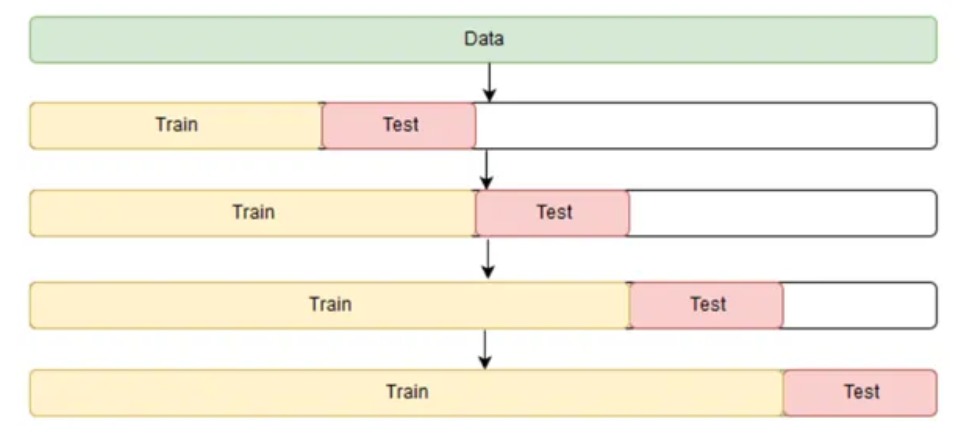
\includegraphics[width=0.65\linewidth]{images/rolling_cv.png}
  \caption{Cross-validation on a Rolling Basis (\cite{time_series_cv}).}
  \label{fig:rolling_cv}
\end{figure}

Figure~\ref{fig:rolling_cv} illustrates the basic idea of cross-validation on a rolling basis. The process starts with a small subset of the data used for training, with the subsequent subset used for testing. The data tested on is then added to the next training set and the subsequent subset is then used for testing. This procedure repeats until the end of the series.

Another approach is blocked cross-validation, where the series is divided into non-overlapping contiguous blocks, each block is used once as a validation set. This method avoids temporal leakage but may be less efficient in utilizing the full dataset compared to rolling schemes \cite{time_series_cv}.

Hyperparameter tuning for RNNs typically involve exploring architectural and training parameters. Important hyperparameter categories and examples include:

\begin{itemize}
    \item \textbf{Network Architecture}: Number of hidden layers, number of neurons per layer.
    \item \textbf{Training Parameters}: Learning rate, optimizer type, batch size, sequence length, gradient clipping thresholds.
    \item \textbf{Regularization}: Dropout probability, weight decay.
\end{itemize}

Strategies such as grid search or random search using cross-validation can be used to explore the hyperparameter space and determine the best combination. The accuracy metrics used to evaluate the models during the cross-validation process is entirely problem dependent, e.g. MSE used for regression, and accuracy for classification

\subsection{\textbf{RNN Limitations}}

While RNNs are powerful tools for time series problems, they suffer from critical limitations, especially when faced with long sequences. The main issue is known as the Vanishing/Exploding Gradient Problem. During backpropagation through time, gradients can either shrink to near zero or grow excessively. This makes it difficult for the network to capture long-term dependencies and can lead to unstable learning. As a result, RNNs often struggle when context from distant time steps is needed to accurately predict the current time step. Mitigations include, gradient clipping, selection of problem appropriate activation functions, better weight initialization, learning rate control, and the use of more advanced architectures like LSTM \cite{rnn_problems}.

\subsection{\textbf{Datasets}}

The recurrent neural networks were trained and evaluated across five distinct regression time series datasets to provide a comprehensive assessment of their performance across diverse tasks.

\subsubsection{\textbf{AMD Stock Data}}

The AMD dataset records AMD (Advanced Micro Devices) stock data over a period of 40 years. The dataset records 10098 instances of 7 variables:

\begin{itemize}
    \item \texttt{Date}: Date the instance was recorded in the format 'yyyy-mm-dd'.
    \item \texttt{Open}: The price at which the stock first traded on the trading day.
    \item \texttt{High}: The highest price the stock reached during the trading day.
    \item \texttt{Low}: The lowest price the stock reached during the trading day.
    \item \texttt{Close}: The final price of the stock when the market closed on that day.
    \item \texttt{Adj Close}: The closing price adjusted for actions like stock splits or dividends.
    \item \texttt{Volume}: The total number of shares traded on the trading day.
\end{itemize}

This is a regression problem, with \texttt{Adj Close} as the response, instead of \texttt{Close}, because it reflects the true economic value of the stock by incorporating adjustments, these adjustments ensure the data more accurately reflects the stock market trends.

\begin{figure}[H]
    \centering
    \includegraphics[width=0.5\textwidth]{images/amd_adj_close.pdf}
    \caption{AMD Adjusted Closing Prices Over Time}
    \label{fig:amd_adj_close}
\end{figure}

Figure~\ref{fig:amd_adj_close} displays how AMD's adjusted closing price fluctuated from 1980 through 2020. The series is clearly non-stationary, with periods of sharp growth and declines. The overall trend is upward, even though there are multiple crashes. Most notably around the early 2000s dot-com bubble and the 2008 financial crisis. The defining upward trend, showing rapid growth, started in 2020.

To formally asses stationarity, and Augmented Dickey-Fuller (ADF) test was conducted. The ADF test is a widely used statistical procedure for detecting unit roots in time series data. If a series has a unit root, it means it behaves like a random walk and is thus non-stationary. The ADF statistic of the AMD stock dataset yielded a p-value of 0.05468, meaning the null hypothesis is not rejected at the 5\% significance level and the series is non-stationary.

The series also exhibits no clear periodic seasonal structure, which is visually evident. Overall the dataset demonstrates the characteristics of a typical non-stationary financial time series, with long-term upward trend, \cite{stock_market_dataset_amd}.

\subsubsection{\textbf{Air Quality}}

The Air Quality dataset records hourly averaged responses of a gas multi-sensor device deployed in an Italian city between March 2004 to February 2005. The dataset records 9358 instances with multiple variables including pollutant concentrations ($CO$, $NMHC$, $C_6H_6$, $NO_x$, $NO_2$), sensor responses from five metal oxide sensors,as well as temperature, relative humidity, and absolute humidity.

For this study the response is  \texttt{CO(GT)}, concentration of carbon monoxide in $mg/m^3$.

\begin{figure}[H]
\centering
\includegraphics[width=0.5\textwidth]{images/air_q_over_time.pdf}
\caption{Air Quality (CO(GT)) Over Time with 24h and 7d Rolling Means}
\label{fig:air_q_over_time}
\end{figure}

Figure~\ref{fig:air_q_over_time} shows the hourly CO(GT) values along with 24-hour and 7-day rolling averages, to see the overall trend more clearly. The raw series is highly volatile, with frequent spikes while the rolling means reveal drifts in the $CO$ concentration over time. These shifts indicate that although the hourly data are noisy, there are underlying patterns driven by human activity and environmental causes.

The dataset is missing some pollutant measurement entries, recorded as placeholder value \textit{-200}, this leads to visible gaps in the series.

\begin{figure}[H]
\centering
\includegraphics[width=0.5\textwidth]{images/air_q_seasonal.pdf}
\caption{Seasonal Decomposition of CO(GT)}
\label{fig:air_q_seasonal}
\end{figure}

Figure~\ref{fig:air_q_seasonal} shows the weekly seasonal decomposition of the \texttt{CO(GT)} series. The trend component highlights longer-term fluctuations, where the average $CO$ levels decrease during mid 2004 and increase again toward late 2004 and early 2005. The seasonal component reveals clear short-term periods, consistent with weekly cycles, possibly linked to human activity.

To assess stationarity an ADF test was done. The test yielded a p-value of $2.498 \times 10^{-16}$, meaning the null hypothesis of the unit root is rejected and the \texttt{CO(GT)} series can be considered stationary. Although the data exhibits short term cycles and noisy behavior, the statistical properties remain stable over time.

In summary the Air Quality dataset exhibits short-term variability, seasonal cycles and a stationary structure. This makes it a suitable candidate for time series modeling with recurrent neural networks, \cite{air_quality}.

\subsubsection{\textbf{Garment Productivity}}

The Garment Productivity dataset records worker productivity across multiple production units in a garment factory over a three month period. It contains 1197 instances of 15 variables that capture operational metrics and contextual information:

\begin{itemize}
    \item \texttt{date}: The date the observation was make, in the format 'yyyy-mmm-dd'.
    \item \texttt{quarter}: Specifies the portion of the month data was collected.
    \item \texttt{department}: Indicates the department of the instance (\textit{sewing or finishing}).
    \item \texttt{day}: Day of the week.
    \item \texttt{team}: Identifier for the production team.
    \item \texttt{targeted\_productivity}: The management determined productivity target (between 0 and 1).
    \item \texttt{smv}: Standard Minute Value, it is the allocated time for a task.
    \item \texttt{wip}: Work-in-Progress, includes the number of unfinished items in the pipeline.
    \item \texttt{over\_time}: Total over-time work.
    \item \texttt{incentive}: Financial incentive allocated to the team.
    \item \texttt{idle\_time}: Time lost due to miscellaneous reasons.
    \item \texttt{idle\_men}: Number of workers who were idle due to production interruption.
    \item \texttt{no\_of\_style\_change}: Number of times the style being produced was changed.
    \item \texttt{no\_of\_workers}: Number of workers in the team.
    \item \texttt{actual\_productivity}: The actual productivity measure achieved by the workers (also between 0 and 1).
\end{itemize}

This dataset combines continuous variables with categorical variables. This distinguishes it from the above mentioned datasets.

\begin{figure}[H]
\centering
\includegraphics[width=0.5\textwidth]{images/actual_prod.pdf}
\caption{Actual Productivity Over Time}
\label{fig:actual_prod}
\end{figure}

Figure~\ref{fig:actual_prod} shows how the average daily productivity changes over time. The plot indicates that the overall trajectory is relatively stable, with fluctuations driven by workload variation, overtime, etc. There appears to be no seasonal pattern, since the data was recorded over a very small window.

An ADF test was conducted to formally investigate stationarity. The test returned a p-value of 0.001457, which is below the 5\% threshold. Thus the garment series is considered stationary, \cite{garment_productivty}.

\subsubsection{\textbf{Electric Production}}

The Electric Production time series records the US Federal Reserve industrial production index for the US electric power sector (series code: IPG2211A2N) over time. It records monthly output of electric power generation, transmission, and distribution. The dataset contains a single feature, \texttt{IPG2211A2N}, recorded at monthly intervals from January 1985 to January 2018.

\begin{figure}[H]
    \centering
    \includegraphics[width=0.5\textwidth]{images/ep_over_time.pdf}
    \caption{Electric Production Over Time}
    \label{fig:ep_over_time}
\end{figure}

Figure~\ref{fig:ep_over_time} indicates the monthly electric production along with 12-month and 36-month rolling means. The series shows an overall upward trend from the mid 1980s to the mid 2000s, with an stagnant period thereafter.

\begin{figure}[H]
    \centering
    \includegraphics[width=0.5\textwidth]{images/ep_seasonal.pdf}
    \caption{Seasonal Decomposition of Electric Production}
    \label{fig:ep_seasonal}
\end{figure}

Figure~\ref{fig:ep_seasonal} shows the yearly seasonal decomposition of the electric production series. It confirms that there is an upward trend from the mid 1980s to mid 2000s with a plateau thereafter. There also appears to be yearly seasonality present in the series, as can be seen in the within-year oscillations in the seasonal component, reflecting seasonal demand in electricity.

And ADF test was conducted that yielded a p-value of 0.1862, which is greater than 0.05. The null hypothesis is rejected hence the series is non-stationary \cite{electric_production}.

\subsubsection{\textbf{Max Planck Institute Weather Data}}

The Weather dataset records meteorological observations at the Max Planck Institute every 10 minutes over the course of one year. The dataset contains 52560 observations of 20 atmospheric variables, which include temperature, air pressure, potential temperature, dew point temperature, relative humidity, vapor pressure measures, specific humidity, water content, air density, wind velocity and direction, as well as radiation and precipitation indicators. 

Temperature (in \si{\celsius}) is the response variable of interest. This dataset thus represents a regression problem where the goal is to forecast the temperature based on other meteorological data.

\begin{figure}[H]
    \centering
    \includegraphics[width=0.5\textwidth]{images/temp_over_time.pdf}
    \caption{Temperature Over Time}
    \label{fig:temp_over_time}
\end{figure}

Figure~\ref{fig:temp_over_time} shows how the observed temperature changed throughout the measurement period. The time series exhibits a seasonal pattern, with temperature increasing from January to July, peaking in the summer months, and then decreasing toward December. This is expected of climactic time series data.

An ADF test was conducted, and yielded a p-value of $2.149e-13$, which is well below the 0.05 significance threshold. This means the series is stationary.

In summary, the dataset provides a comprehensive representation of atmospheric conditions and demonstrates the dynamics of meteorological processes, where the response variable (temperature) is influenced by multiple interacting environmental factors \cite{weather_dataset}.

\section{\textbf{Implementation}}

\subsection{\textbf{Technology Stack}}
All code was implemented in Python 3.12 using the following stack:
\begin{itemize}
    \item \textbf{Core Numerics}: \texttt{numpy}
    \item \textbf{Data Wrangling}: \texttt{pandas}
    \item \textbf{Time Series Utilities}: \texttt{statsmodels}
    \item \textbf{Visualization}: \texttt{matplotlib}
    \item \textbf{Preprocessing}: \texttt{scikit-learn}
    \item \textbf{Modeling}: \texttt{pytorch}
\end{itemize}

\subsection{\textbf{RNN Architectures}}
The RNNs investigated in this study were implemented using the PyTorch API. PyTorch is a highly customizable open-source deep learning framework. Each RNN type was defined as a custom \texttt{nn.Module} class, with a forward pass implementation tailored to the recurrence formula of the relevant architecture.
\begin{itemize}
    \item \textbf{ElmanRNN}: A tanh PyTorch default RNN cell (\texttt{nn.RNN}) followed by a linear output layer.
    \item \textbf{JordanRNN}: Forward pass implements the output-hidden state recurrence. The previous output is passed through an activation function (\texttt{identity}/\texttt{sigmoid}/\texttt{softmax}/\texttt{tanh}) and then fed into the hidden layer at the current time step via a learned projection.
    \item \textbf{MultiRNN}: Implemented as a hybrid of the Elman and Jordan architectures, combining hidden-to-hidden and output-to-hidden recurrence.
\end{itemize}
Implementations were parameterized, which allows users to choose hidden layer size, output activation function, and output type (sequence-to-one vs. sequence-to-sequence). The implementations also included gradient clipping to prevent the exploding/vanishing gradient problem.

All model implementations use the \texttt{tanh} hidden activation function and a final linear layer for regression outputs.

\subsection{\textbf{Training Utilities \& Pipeline}}
To keep code modular and compact, a set of utilities that encapsulates the steps in the model training pipeline were implemented:
\begin{itemize}
    \item \textbf{Sequence building}: \texttt{make\_sequences} converts $(X,y)$ into fixed-length windows and forecast horizon aligned targets.
    \item \textbf{Datasets \& loaders}: \texttt{TimeSeriesDataset} wraps sequences as tensors. \texttt{DataLoaders} are created without shuffling (respecting temporal order) and without dropping tail batches.
    \item \textbf{Model factory}: \texttt{create\_model} constructs the requested model with the required architecture and parameters and moves it to the selected device (CPU/GPU).
    \item \textbf{Epoch routines}: \texttt{train\_one\_epoch} and \texttt{evaluate\_one\_epoch} standardize the train/validation passes, apply gradient clipping, and accumulate loss in an epoch size weighted manner across a single epoch.
    \item \textbf{Early stopping}: \texttt{fit\_early\_stopping} tracks the best validation loss, snapshots weights, and halts on \texttt{patience}. The best state dict is restored before evaluation.
    \item \textbf{Scaling helpers}: \texttt{fit\_seq\_scalers} and \texttt{transform\_seq} fit \texttt{MinMaxScalers} on the training data only and then transforms relevant descriptive features and targets.
    \item \textbf{Prediction}: \texttt{predict\_all} performs batched inference.
\end{itemize}

\subsection{\textbf{Cross-Validation}}
The cross-validation process for hyperparameter tuning is handled by:
\begin{itemize}
    \item \textbf{Windowing}: \texttt{rolling\_windows} yields chronological (train, val) index slices with a user-defined train size, validation size, and step.
    \item \textbf{Hyperparameter config scoring}: \texttt{ts\_cv\_score} takes a model, fits scalers on each train slice, performs training with early stopping, inverse-transforms predictions, and returns per-fold scores and their summary stats.
    \item \textbf{Grid search}: \texttt{grid\_search\_ts\_cv} iterates over a hyperparameter configuration grid for a given architecture, invokes \texttt{ts\_cv\_score}, and selects the configuration with minimal mean CV error.
\end{itemize}

\subsection{\textbf{Final Model Training}}
Final model training and evaluation logic is encapsulated in:
\begin{itemize}
    \item \textbf{fit\_best}: given the selected hyperparameter configuration and training data, it creates a small validation dataset for internal early stopping, fits scalers on the remaining training sequences, restores best weights, performs test inference, and inverse-transforms outputs.
    \item \textbf{Metrics}: metric functions (\texttt{RMSE}, \texttt{MAE}, \texttt{R2}) are passed as a dictionary, computed on original response units, and returned alongside predictions for downstream plotting or tables.
    \item \textbf{Experiment driver}: \texttt{run\_experiments} loops over horizons and architectures, applies grid search and \texttt{fit\_best}, and collects results.
\end{itemize}

\section{\textbf{Empirical process}}

\subsection{\textbf{Objective}}
The objective of this study was to compare three simple recurrent neural network architectures, namely the Elman, Jordan and Multi-RNN, in the context of five different time series forecasting problems. Five real-world regression time series datasets were selected that represent a diverse range of temporal patterns, stationarity, and application domains.
The central aim of the study was to evaluate the relative strengths and weaknesses of the Elman, Jordan, and Multi-RNN architectures across different forecasting horizons, and to test whether the performance ranking of these models is consistent across various datasets or whether certain architectures are better suited to specific types of time series.
Feature standardization, sequence construction, training setup, and evaluation procedures ensure the empirical process was designed to isolate the effect of model architecture as the key property of interest under investigation.

\subsection{\textbf{Dataset Specific Preprocessing}}
\subsubsection{\textbf{AMD Stock Data}}
\begin{itemize}
    \item \texttt{Adj Close} was chosen as response, hence the redundant column \texttt{Close} was dropped.
    \item Rows with zero-valued opening prices were removed as these entries are most likely data entry errors, and there are only a few of them so removing them will not introduce any major bias into the dataset.
\end{itemize}

\subsubsection{\textbf{Air Quality}}
\begin{itemize}
    \item Several fields use the place holder value \textit{-200} to indicate sensor failures. These values were treated as missing entries.
    \item Records missing an observation for the response \texttt{CO(GT)} were completely dropped.
    \item The dataset contains five sensor readings \texttt{PT08.S1(CO)}, \texttt{PT08.S2(NMHC)}, \texttt{PT08.S3(NOx)}, \texttt{PT08.S4(NO2)}, \texttt{PT08.S5(O3)}, and three meteorological variables \texttt{T}, \texttt{RH}, \texttt{AH}. It was found that the missing entries in these features were co-located. These rows were entirely removed from the dataset as they contained mostly missing values.
    \item Other missing values were interpolated using time-based interpolation, using the timestamp index to interpolate values between the nearest known points in time.
\end{itemize}

\subsubsection{\textbf{Garment Productivity}}
\begin{itemize}
    \item Invalid entries, such as entries missing key fields such as \texttt{date} or \texttt{actual\_productivity} (response) were removed.
    \item The \texttt{wip} column was entirely removed from the dataset, as it was missing half of its entries.
    \item The dataset contains a mix of numeric and categorical features. The categorical variables were converted into one-hot-encoded vectors using dummy encodings. This makes the categorical features usable in neural network based models.
\end{itemize}

\subsubsection{\textbf{Electric Production}}
No preprocessing needed to be done on the Electric Production dataset as it is a complete dataset containing no missing values or invalid entries.

\subsubsection{\textbf{Max Planck Institute Weather Data}}
No preprocessing was needed for this dataset either.

\subsection{\textbf{Dataset Agnostic Preprocessing}}
\subsubsection{\textbf{Scaling}}
For all datasets, the descriptive and response features were normalized using scikit-learn's \texttt{MinMaxScaler}. During cross-validation and final model training, the scalers were fit on the training data only and then applied to the corresponding training, test and/or validation sets. This was done to prevent information from future time steps to leak into past time steps.

The \texttt{MinMaxScaler} was used because the RNN implementations use the tanh hidden activation function, which outputs values in the range [-1, 1]. By scaling inputs and outputs into compatible ranges, the model training process was more stable, which reduced the risk of vanishing or exploding gradients.

\subsubsection{\textbf{Sequence Construction}}
Each dataset was transformed into sequences of fixed length. This allowed the recurrent neural networks to receive a window of past observations as inputs and predict future values at specified horizons.

A sliding window procedure was used to construct the sequences. First the datasets were sorted by time stamp, and then for a given window length \texttt{L}, a contiguous block of \texttt{L} timesteps was extracted as an input sequence, and a value at a specified horizon was selected as the target. By moving the window forward one step at a time, multiple overlapping sequences were generated.

A moderate sequence length of 30 items was selected as this effectively balances temporal context while keeping compute costs manageable. The earlier items in longer sequences would be wastefully included, as their temporal information will be lost by overly extensive recurrence.

The study considered multiple horizons to evaluate the models' short-term and long-term predictive performance. Specifically predictions were made for horizons of 1, 3, 5, and 7 time steps ahead.

To clarify:
\begin{itemize}
    \item \textbf{Horizon = 1}: If the sequence length is 3 and the time series is \texttt{[1, 2, 3, 4, 5, 6, 7]}, then the input sequence is \texttt{[1, 2, 3]} and the target is \texttt{4}. This is simple next-item prediction.
    \item \textbf{Horizon = 3}. Under the same conditions, the input sequence would be \texttt{[1, 2, 3]} and the target is \texttt{6}
\end{itemize}
The models were trained in a sequence-to-one configuration, where each input sequence of 30 timesteps were used to predict a single output at the specified horizon. This allowed a fair comparison of Elman, Jordan, and Multi-RNN models across multiple datasets.

\subsection{\textbf{Model Training}}
After dataset preprocessing, the models were trained using a training setup that was designed to ensure stable learning, prevent overfitting, and allow for fair comparison of the three RNN model architectures across five different regression time series datasets.

\subsubsection{\textbf{Loss Function}}
All models were optimized using the Mean Squared Error loss function. This loss function is a common choice for regression problems, as it directly measures the squared deviation between predicted and true values, as well as being differentiable which is important for neural networks using gradient descent.

\subsubsection{\textbf{Optimization Algorithm}}
All models were trained using the Adam optimizer. The Adam optimizer (Adaptive Moment Estimation) is one of the most popular optimization algorithms used in training neural networks. It combines momentum, to smooth parameter updates by incorporating information from past gradients, and adaptive learning rate, to adjust step size of each parameter dynamically based on the history of gradients.

\subsubsection{\textbf{Regularization \& Stability Measures}}
To prevent overfitting and stabilize training, the following steps were taken:
\begin{itemize}
    \item \textbf{Weight Decay}: Incorporated in optimizer to penalize overly large weights and improve generalization.
    \item \textbf{Gradient Clipping}: A threshold was applied to the gradient during backpropagation, to clip the gradient and prevent instability during training.
    \item \textbf{Model Capacity Tuning}: Hidden layer size was included as a hyperparameter to be tuned during cross-validation, and sizes were varied to find the optimal hidden layer size for each model.
\end{itemize}

\subsubsection{\textbf{Early Stopping}}
Another measure taken to prevent overfitting was to use an early stopping mechanism when training the models. Training was halted when validation loss failed to improve after a fixed patience period (ranging from 8 to 12 epochs). At termination, the model parameters corresponding to the lowest validation loss were chosen as the optimal parameter set.

\subsubsection{\textbf{Batching and Data Loading}}
Input sequences were grouped into mini-batches using PyTorch's \texttt{DataLoader}. Batch sizes varied from 256 to 512 depending on the hyperparameter set being evaluated.

\subsubsection{\textbf{Hyperparameter Grid}}
A hyperparameter grid was used to tune the hyperparameters of each of the models during cross validation. The grid included the following parameters:
\begin{itemize}
    \item Hidden layer size: 32-256 units
    \item Learning rate: $1e-3$ to $5e-5$
    \item Batch size: 256 and 512
    \item Epochs: 60-120
    \item Patience for early stopping: 8-12
    \item Weight decay: $0$ to $1e-4$
\end{itemize}

\subsubsection{\textbf{Cross-Validation and Model Selection}}
Time series cross-validation was used to select optimal hyperparameters while respecting temporal order. After sequence construction the data was chronologically split (80/20) into a training portion and a test portion. The training portion was used to form rolling windows comprising of (train, validation) slices:
\begin{enumerate}
    \item For each window, \texttt{MinMaxScalers} were fit on the train slice only, and then applied to the validation slice to prevent data leakage.
    \item For each RNN architecture and hyperparameter configuration from the grid, a model was trained on the train slice and evaluated on the validation slice using RMSE computed on the original response scale.
    \item The cross-validation score for a model configuration was calculated as the mean RMSE across all rolling windows (folds).
\end{enumerate}
For each dataset, model and forecast horizon ([1, 3, 5, 7]), the hyperparameter configuration with the lowest mean CV RMSE was selected as the best hyperparameter configuration for that architecture, dataset, and forecast horizon. This process ensured a fair comparison driven only in difference between model architecture.

\subsubsection{\textbf{Final Model Training}}
Given the optimal hyperparameter set for a model architecture, forecast horizon, and dataset, final model training proceeded as follows:
\begin{enumerate}
    \item Within the entire training portion of the dataset, a small chronological tail (10\%) was reserved as a validation set to be used for early stopping.
    \item \texttt{MinMaxScalers} were then fit on the remaining training data.
    \item The model was then trained with MSE loss, and the Adam optimizer, using gradient clipping and weight decay where applicable.
\end{enumerate}

\subsection{\textbf{Final Model Evaluation}}
To provide an representative view of model performance and fit, three regression metrics were calculated for each model on the test data set:
\begin{itemize}
    \item \textbf{RMSE}: Squared error.
    \item \textbf{MAE} Average absolute deviation.
    \item \boldmath{$R^2$} Explained variance.
\end{itemize}
Evaluating these metrics across the different models and forecast horizons reveal how the architectures perform compared to each other, and how they trade off short-term precision with long-range stability.

\subsection{\textbf{Reproducibility}}
To ensure reproducibility all random seeds were set consistently for NumPy and PyTorch. Nvidia CUDA deterministic flags were enabled where applicable.

\section{\textbf{Results \& discussion}}
As mentioned, this study evaluates three recurrent neural network architectures - Elman, Jordan, and Multi-RNN - across five time series regression problems. All tasks involve predicting a continuous response, thus evaluation focusses on regression metrics.

Root Mean Squared Error (RMSE) is used during cross-validation as the primary model selection criterion because it penalizes large discrepancies between actual and predicted targets more strongly than Mean Absolute Error (MAE).

On the test set, model performance is evaluated with RMSE, MAE, and $R^2$. RMSE reflects variance weighted accuracy, MAE captures the average magnitude of error and $R^2$ measures how well the model explains the variability of the response.

\subsection{\textbf{AMD Stock Data}}
The first problem concerns forecasting AMD's adjusted closing stock price from open, high, low, and volume observations. Stock price data are inherently non-stationary, which makes prediction challenging.

The RNN models were trained to predict the adjusted closing price $h$ steps ahead, for forecast horizons in $h \in [1,3,5,7]$.

\begin{table}[H]
\centering
\caption{AMD model performance ($h=1$).}
\label{tab:amd_h1}
\begin{tabular}{lcccc}
\toprule
\textbf{Model} & \textbf{CV RMSE} & \textbf{Test RMSE} & \textbf{Test MAE} & $\mathbf{R^2}$ \\
\midrule
Elman  & 0.5837 & 1.1529 & 0.5750 & 0.9907 \\
Jordan & 0.5319 & 1.2662 & 0.6165 & 0.9888 \\
Multi  & 0.4863 & 1.5580 & 0.8101 & 0.9831 \\
\bottomrule
\end{tabular}
\end{table}

\begin{table}[H]
\centering
\caption{AMD model performance ($h=3$).}
\label{tab:amd_h3}
\begin{tabular}{lcccc}
\toprule
\textbf{Model} & \textbf{CV RMSE} & \textbf{Test RMSE} & \textbf{Test MAE} & $\mathbf{R^2}$ \\
\midrule
Elman  & 0.8307 & 1.1507 & 0.6134 & 0.9908 \\
Jordan & 0.7913 & 1.4183 & 0.7106 & 0.9860 \\
Multi  & 0.7601 & 1.3528 & 0.7197 & 0.9872 \\
\bottomrule
\end{tabular}
\end{table}

\begin{table}[H]
\centering
\caption{AMD model performance ($h=5$).}
\label{tab:amd_h5}
\begin{tabular}{lcccc}
\toprule
\textbf{Model} & \textbf{CV RMSE} & \textbf{Test RMSE} & \textbf{Test MAE} & $\mathbf{R^2}$ \\
\midrule
Elman  & 1.0310 & 1.9398 & 1.0958 & 0.9737 \\
Jordan & 0.9821 & 1.9406 & 0.9461 & 0.9737 \\
Multi  & 0.9895 & 1.8280 & 0.9197 & 0.9767 \\
\bottomrule
\end{tabular}
\end{table}

\begin{table}[H]
\centering
\caption{AMD model performance ($h=7$).}
\label{tab:amd_h7}
\begin{tabular}{lcccc}
\toprule
\textbf{Model} & \textbf{CV RMSE} & \textbf{Test RMSE} & \textbf{Test MAE} & $\mathbf{R^2}$ \\
\midrule
Elman  & 1.1770 & 2.1858 & 1.2403 & 0.9667 \\
Jordan & 1.1447 & 2.0999 & 1.0789 & 0.9692 \\
Multi  & 1.1282 & 1.7695 & 0.9845 & 0.9781 \\
\bottomrule
\end{tabular}
\end{table}

For short to medium horizons ($h$ = 1 \& $h$ = 3), the Elman model overall performs the best. Across both horizons it maintains the lowest RMSE and MAE, and hightest $R^2$ values, despite having the largest CV RMSE. In both cases the Multi-RNN attains the best CV RMSE, but underperforms when compared to the Elman model on the test set. This suggests mild overfitting present in the Multi-RNN model. The simpler Elman architecture, which relies solely on hidden state recurrence, generalizes best when the forecast is only a few time steps ahead.

For medium to longer horizons ($h$ = 5 \& $h$ = 7), the Multi-RNN model becomes the best performing model. It maintains the lowest RMSE, MAE and highest $R^2$ values relative to the other two models, while also still maintaining the lowest CV RMSE score. This suggest that the inclusion of both hidden state and output recurrence allows the Multi-RNN model to more accurately capture medium-to-long range dependencies in temporal data, causing the model to have more accurate predictions as the target moves further away from the immediate next step.

For all model architectures, as the forecast horizon increases, RMSE and MAE increase and $R^2$ declines, reflecting error accumulation as forecast horizon increases. The Elman RNN dominates at short horizons, but the Multi-RNN performs best as the horizon increases, suggesting that the inclusion of the Jordan recurrence becomes helpful once short-term patterns fade and models need to rely on longer-term trends. The Jordan architecture remains competitive but does not provide any clear advantage.

The results obtained in the setup of predicting raw price levels highlights the trade-off between simple models that generalize well at short-horizons and more complex models that capture long-range patterns.  

\subsection{\textbf{Air Quality}}
The focus of the Air Quality problem is to predict \texttt{CO(GT)} pollutant concentration at different forecast horizons given an input sequence of sensor measurements and meteorological metric data at contiguous time steps.

The Elman, Jordan, and Multi-RNN models under investigation were trained to predict across the same horizons as the AMD Stock Data, $h \in [1,3,5,7]$.

\begin{table}[H]
\centering
\caption{Air Quality model performance ($h$=1)}
\label{tab:aq_h1}
\begin{tabular}{lcccc}
\toprule
\textbf{Model} & \textbf{CV RMSE} & \textbf{Test RMSE} & \textbf{MAE} & \(\mathbf{R^2}\) \\
\midrule
Elman  & 0.9493 & 0.7685 & 0.6014 & 0.6518 \\
Jordan & 0.9652 & 0.7634 & 0.5868 & 0.6564 \\
Multi  & 0.9331 & 0.7781 & 0.5943 & 0.6430 \\
\bottomrule
\end{tabular}
\end{table}

\begin{table}[H]
\centering
\caption{Air Quality model performance ($h$=3)}
\label{tab:aq_h3}
\begin{tabular}{lcccc}
\toprule
\textbf{Model} & \textbf{CV RMSE} & \textbf{Test RMSE} & \textbf{MAE} & \(\mathbf{R^2}\) \\
\midrule
Elman  & 1.3571 & 1.2542 & 0.9434 & 0.0726 \\
Jordan & 1.4823 & 1.2415 & 0.9284 & 0.0913 \\
Multi  & 1.3412 & 1.2503 & 0.9708 & 0.0783 \\
\bottomrule
\end{tabular}
\end{table}

\begin{table}[H]
\centering
\caption{Air Quality model performance ($h$=5)}
\label{tab:aq_h5}
\begin{tabular}{lcccc}
\toprule
\textbf{Model} & \textbf{CV RMSE} & \textbf{Test RMSE} & \textbf{MAE} & \(\mathbf{R^2}\) \\
\midrule
Elman  & 1.4525 & 1.3229 & 1.0303 & -0.0318 \\
Jordan & 1.6336 & 1.3023 & 1.0274 & 0.0001 \\
Multi  & 1.4277 & 1.3174 & 1.0528 & -0.0232 \\
\bottomrule
\end{tabular}
\end{table}

\begin{table}[H]
\centering
\caption{Air Quality model performance ($h$=7)}
\label{tab:aq_h7}
\begin{tabular}{lcccc}
\toprule
\textbf{Model} & \textbf{CV RMSE} & \textbf{Test RMSE} & \textbf{MAE} & \(\mathbf{R^2}\) \\
\midrule
Elman  & 1.4771 & 1.2671 & 0.9964 & 0.0534 \\
Jordan & 1.6571 & 1.3178 & 1.0382 & -0.0239 \\
Multi  & 1.4435 & 1.2039 & 0.9502 & 0.1455 \\
\bottomrule
\end{tabular}
\end{table}

As forecast horizon increases, performance degrades for each model, which is consistent with rising uncertainty at longer horizons.

At short to medium horizons ($h=1$ \& $h=3$), the Jordan model performs the best, delivering the lowest Test RMSE and MAE with the highest $R^2$, despite higher CV RMSE scores than the other models. This might suggest (although not likely) benign overfitting, which means that the Jordan model might generalize better under less regularization and overfitting protection.

For medium horizons $h=5$, Jordan still remains the top performing model on the test set. Notably, $R^2$ drops sharply as the forecast horizon increases from $h=1$ to $h=3$, and hovers around zero when increased to $h=5$, with negative $R^2$ values for the Elman and Multi-RNN models. This indicates that simple mean predictions become difficult to outperform as the horizon grows.

At the longest horizon $h=7$, the Multi-RNN model performs significantly better than both the Elman and Jordan RNN models. This aligns with previous findings that including both Elman and Jordan recurrences to create a more complex model better captures long-term temporal relations.

The models attain relatively high $R^2$ for immediate next-item prediction, which degrades as the forecast horizon increases, consistent with reduced predictability of pollutant concentration at longer horizons. From short to medium  horizons $R^2$ falls sharply, with a modest rebound at longer horizons for the Multi-RNN model suggesting that more complex architectures can mitigate long horizon degradation.

The Jordan RNN performs best at short and medium horizons, with the Multi-RNN model performing best at longer horizons. The Elman architecture remains competitive but provides no distinct advantage.

Air quality time series data typically exhibit strong short term correlation, pollutant levels between contiguous time steps are highly related. This means that at short forecast horizons, like next-step prediction, the local persistence of pollutant levels make prediction comparatively easy. As horizons grow, uncertainty compounds and prediction becomes harder.

\subsection{\textbf{Garment Productivity}}
The Garment Productivity problem concerns forecasting worker productivity from shop floor signals. The models were trained and evaluated across multiple forecast horizons, $h \in [1,3,5,7]$.

\begin{table}[H]
\centering
\caption{Garment Productivity model performance ($h=1$).}
\label{tab:gp_h1}
\begin{tabular}{lcccc}
\toprule
\textbf{Model} & \textbf{CV RMSE} & \textbf{Test RMSE} & \textbf{Test MAE} & $\mathbf{R^2}$ \\
\midrule
Elman  & 0.1628 & 0.1676 & 0.1184 & -0.1375 \\
Jordan & 0.1774 & 0.1818 & 0.1377 & -0.3377 \\
Multi  & 0.1675 & 0.1712 & 0.1210 & -0.1862 \\
\bottomrule
\end{tabular}
\end{table}

\begin{table}[H]
\centering
\caption{Garment Productivity model performance ($h=3$).}
\label{tab:gp_h3}
\begin{tabular}{lcccc}
\toprule
\textbf{Model} & \textbf{CV RMSE} & \textbf{Test RMSE} & \textbf{Test MAE} & $\mathbf{R^2}$ \\
\midrule
Elman  & 0.1650 & 0.1641 & 0.1287 & -0.0854 \\
Jordan & 0.1849 & 0.2148 & 0.1494 & -0.8602 \\
Multi  & 0.1688 & 0.1703 & 0.1243 & -0.1693 \\
\bottomrule
\end{tabular}
\end{table}

\begin{table}[H]
\centering
\caption{Garment Productivity model performance ($h=5$).}
\label{tab:gp_h5}
\begin{tabular}{lcccc}
\toprule
\textbf{Model} & \textbf{CV RMSE} & \textbf{Test RMSE} & \textbf{Test MAE} & $\mathbf{R^2}$ \\
\midrule
Elman  & 0.1662 & 0.1685 & 0.1329 & -0.1451 \\
Jordan & 0.1834 & 0.1682 & 0.1338 & -0.1400 \\
Multi  & 0.1717 & 0.1986 & 0.1479 & -0.5907 \\
\bottomrule
\end{tabular}
\end{table}

\begin{table}[H]
\centering
\caption{Garment Productivity model performance ($h=7$).}
\label{tab:gp_h7}
\begin{tabular}{lcccc}
\toprule
\textbf{Model} & \textbf{CV RMSE} & \textbf{Test RMSE} & \textbf{Test MAE} & $\mathbf{R^2}$ \\
\midrule
Elman  & 0.1711 & 0.1717 & 0.1446 & -0.1882 \\
Jordan & 0.1829 & 0.1685 & 0.1240 & -0.1447 \\
Multi  & 0.1709 & 0.1809 & 0.1367 & -0.3186 \\
\bottomrule
\end{tabular}
\end{table}

Across all forecast horizons the usual degradation of model performance is present, but it is much more pronounced on the Garment Productivity dataset because the response productivity measure is a proportion in the range [0, 1].

For next-item prediction ($h=1$), the Elman RNN performs the best, it has the lowest RMSE, and MAE metric values with the highest $R^2$ value. All models have negative $R^2$ values which mean that they all perform worse than a model just predicting the mean productivity for each input sequence.

For medium forecast horizons ($h=3$ \& $h=5$), the Elman network still performs the best. Test RMSE and MAE for all models degrade as the horizon increases from short to medium, except the Jordan RNN, its performance actually increases as the forecast horizon increases, and at a horizon of $h=5$ the Elman and Jordan model effectively perform the same. Notably Test MAE takes on values in the range [0.1, 0.15], which means that predictions are off by $\sim 12.5\%$ on average, which is not very good.

At the longest horizon ($h=7$), the Jordan RNN performs the best. It has the lowest RMSE and MAE scores with the highest $R^2$ score. All models still have negative $R^2$ values which mean that they still perform worse than predicting the mean.

All models perform poorly, the model's predictions are off on average by 0.125 units, and since the response is in the range [0, 1] this is quite a large error. Further all $R^2$ values, across model architectures and forecast horizons, are negative meaning all models perform worse than just predicting the mean of \texttt{actual\_productivity} for each input sequence.

For short forecast horizons the Elman RNN performs best, for medium horizons, there is no real difference between the performance of the Elman and Jordan RNN, but at long forecast horizons the Jordan model performs best, although it is important to note that no RNN model actually performs well in an absolute sense. The Multi-RNN model provides no distinct advantage for this problem.

Garment productivity is hard to forecast because the garment manufacturing process is driven by short-memory, and regime changes (style switches, SMV shifts, incentives) that cause abrupt jumps rather than smooth trends. This means the RNN models are not able to accurately capture any temporal patterns present in the data.

\subsection{\textbf{Electric Production}}

The Electric Production problem concerns predicting US industrial electric power production based on an input sequence of previous electric production measurements. This is the simplest problem investigated as it contains measurements of only a single variable. Like the models before, the RNN models trained on the Electric Production dataset were evaluated at horizons $h \in [1,3,5,7]$.

\begin{table}[H]
\centering
\caption{Electric Production model performance ($h=1$).}
\label{tab:ep_h1}
\begin{tabular}{lcccc}
\toprule
\textbf{Model} & \textbf{CV RMSE} & \textbf{Test RMSE} & \textbf{Test MAE} & $\mathbf{R^2}$ \\
\midrule
Elman  & 9.9853  & 10.6117 & 8.7759 & -0.2229 \\
Jordan & 10.4397 & 7.9953  & 6.2540 & 0.3058 \\
Multi  & 6.3614  & 4.2711  & 3.4017 & 0.8019 \\
\bottomrule
\end{tabular}
\end{table}

\begin{table}[H]
\centering
\caption{Electric Production model performance ($h=3$).}
\label{tab:ep_h3}
\begin{tabular}{lcccc}
\toprule
\textbf{Model} & \textbf{CV RMSE} & \textbf{Test RMSE} & \textbf{Test MAE} & $\mathbf{R^2}$ \\
\midrule
Elman  & 10.3303 & 7.3707  & 6.0734 & 0.4162 \\
Jordan & 10.3370 & 12.2193 & 10.2021 & -0.6046 \\
Multi  & 6.3953  & 6.5294  & 4.9870 & 0.5418 \\
\bottomrule
\end{tabular}
\end{table}

\begin{table}[H]
\centering
\caption{Electric Production model performance ($h=5$).}
\label{tab:ep_h5}
\begin{tabular}{lcccc}
\toprule
\textbf{Model} & \textbf{CV RMSE} & \textbf{Test RMSE} & \textbf{Test MAE} & $\mathbf{R^2}$ \\
\midrule
Elman  & 9.5779  & 9.1306  & 7.6675 & 0.1041 \\
Jordan & 10.4779 & 12.3032 & 9.8914 & -0.6268 \\
Multi  & 4.7539  & 7.0623  & 5.2254 & 0.4640 \\
\bottomrule
\end{tabular}
\end{table}

\begin{table}[H]
\centering
\caption{Electric Production model performance ($h=7$).}
\label{tab:ep_h7}
\begin{tabular}{lcccc}
\toprule
\textbf{Model} & \textbf{CV RMSE} & \textbf{Test RMSE} & \textbf{Test MAE} & $\mathbf{R^2}$ \\
\midrule
Elman  & 9.5051 & 10.3615 & 8.5946 & -0.1538 \\
Jordan & 8.3729 & 9.3305  & 7.4672 & 0.0644 \\
Multi  & 7.7781 & 5.3698  & 3.7958 & 0.6901 \\
\bottomrule
\end{tabular}
\end{table}

Across all horizons, the Multi-RNN models dominate over the Elman and Jordan models. They maintain the lowest RMSE and MAE values, with the highest $R^2$ values. For some of the forecast horizons, the Elman and Jordan models actually perform worse than predicting the mean, while the Mulit-RNN model remains competitive across all horizons.

The degradation of model performance is present as horizon increases, but from $h=5$ to $h=7$ the Jordan and Multi-RNN models have quite a positive jump in performance. The Multi-RNN model still dominates, but this suggests that the output-to-hidden recurrence might help the Multi-RNN model more accurately model seasonal information present at longer forecast horizons.

Overall the Multi-RNN model performs best, consistently maintaining best test metric scores and lowest cross-validation scores, suggesting the model balances performance with complexity very well. Relative to the Multi-RNN model, the Elman and Jordan models offer no benefits and often perform no better than naive baselines.

The Multi-RNN model performs best on the Electric Production dataset because it blends hidden-to-hidden and output-to-hidden recurrences to capture trend \& seasonality along with most recent predictions to prevent error accumulation. This blend of Elman and Jordan recurrences make the Multi-RNN model more capable of accurately capturing the rich temporal nature, seasonality, and trend of the Electric Production dataset.

\subsection{\textbf{Max Planck Institute Weather Data}}

The Weather Dataset concerns predicting the temperature given other atmospheric variables. This is the most complex problem investigated as it contains 52560 observations of 20 variables. RNN models were trained on the same forecast horizons as all other problems: $h \in [1,3,5,7]$.

\begin{table}[H]
\centering
\caption{Weather model performance ($h=1$).}
\label{tab:wx_h1}
\begin{tabular}{lcccc}
\toprule
\textbf{Model} & \textbf{CV RMSE} & \textbf{Test RMSE} & \textbf{Test MAE} & $\mathbf{R^2}$ \\
\midrule
Elman  & 0.2568 & 0.3255 & 0.2523 & 0.9957 \\
Jordan & 0.2212 & 0.2630 & 0.2002 & 0.9972 \\
Multi  & 0.2342 & 0.2076 & 0.1558 & 0.9983 \\
\bottomrule
\end{tabular}
\end{table}

\begin{table}[H]
\centering
\caption{Weather model performance ($h=3$).}
\label{tab:wx_h3}
\begin{tabular}{lcccc}
\toprule
\textbf{Model} & \textbf{CV RMSE} & \textbf{Test RMSE} & \textbf{Test MAE} & $\mathbf{R^2}$ \\
\midrule
Elman  & 0.5121 & 0.4303 & 0.3277 & 0.9926 \\
Jordan & 0.5047 & 0.5471 & 0.4427 & 0.9880 \\
Multi  & 0.4959 & 0.3764 & 0.2671 & 0.9943 \\
\bottomrule
\end{tabular}
\end{table}

\begin{table}[H]
\centering
\caption{Weather model performance ($h=5$).}
\label{tab:wx_h5}
\begin{tabular}{lcccc}
\toprule
\textbf{Model} & \textbf{CV RMSE} & \textbf{Test RMSE} & \textbf{Test MAE} & $\mathbf{R^2}$ \\
\midrule
Elman  & 0.7375 & 0.5994 & 0.4559 & 0.9856 \\
Jordan & 0.7199 & 0.7453 & 0.6048 & 0.9777 \\
Multi  & 0.7051 & 0.7606 & 0.6145 & 0.9768 \\
\bottomrule
\end{tabular}
\end{table}

\begin{table}[H]
\centering
\caption{Weather model performance ($h=7$).}
\label{tab:wx_h7}
\begin{tabular}{lcccc}
\toprule
\textbf{Model} & \textbf{CV RMSE} & \textbf{Test RMSE} & \textbf{Test MAE} & $\mathbf{R^2}$ \\
\midrule
Elman  & 0.9327 & 1.0127 & 0.8131 & 0.9588 \\
Jordan & 0.9847 & 0.8801 & 0.6873 & 0.9689 \\
Multi  & 0.8481 & 0.8113 & 0.6366 & 0.9736 \\
\bottomrule
\end{tabular}
\end{table}

For the shortest horizon ($h=1$), the Multi-RNN achieves the best scores across all metrics (lowest RMSE/MAE, highest $R^2$), followed by Jordan, then Elman. All models remain competent and explain $> 99\%$ of the variance present in the data. This means that for next-item prediction any one of Elman, Jordan, or Multi-RNN models will yield excellent performance, with Mulit-RNN slightly outperforming the other two.

For medium horizons ($h=3$), all models remain competitive, with Mulit-RNN still performing the best. Even at medium forecast horizons the models explain $>98.8\%$ of the variance in the data and maintain RMSE and MAE scores less than one unit.

For $h=5$ the trend shifts, the Elman model performs best at a forecast horizon of 5. All models deteriorate from $h=3$ to $h=5$, but the Elman model has the least severe degradation in performance. All RNN models still explain $> 97.7\%$ of the variance in the dataset and maintain RMSE and MAE scores less than one unit.

At the longest horizon ($h=7$), the Multi-RNN model again performs the best, with Jordan following, and Elman performing the worst. Again all models degrade in performance as the forecast horizon increases, but Elman degrades the most.

Overall the Multi-RNN dominates at very short and long horizons due to its two memory pathways (internal state that preserves seasonal phase and trend \& correction loop incorporating recent outputs), while Elman exhibits strong performance at medium horizons, but lacks the corrective pathway to excel at longer horizons. Jordan is competitive for next-item prediction, but tends to underperform consistently over longer horizons as errors compound.

As horizon increases, RMSE and MAE generally grow and $R^2$ declines, reflecting the expected accumulation of uncertainty. Nonetheless, all models retain very high $R^2$ at short horizons ($>0.99$ at $h{=}1$) and remain strong even at $h{=}7$, indicating a predictable signal at the 10-minute cadence.

Temperature at 10-minute measurement intervals exhibit strong short-range correlation, this means that output-to-hidden feedback in Jordan and Multi-RNN models effectively leverage persistence, but the Multi-RNN maintains hidden context which aids it as the forecast horizon grows. The Multi-RNN's complexity is well matched to the data volume ($> 50000$ observations), allowing it to learn richer dynamics, like the seasonality and overall trend.

In summary for short and long horizons the Multi-RNN model performs best, while the Elman RNN can be more reliable at medium horizons.

\section{\textbf{Conclusion}}

This study set out to compare three simple recurrent neural network architectures - Elman, Jordan, and Multi-RNN - across five real-world regression time series forecasting tasks and multiple horizons. By standardizing preprocessing, rolling cross-validation, and training protocols, the analysis isolated architectural effects on model performance.

The results show that no single RNN variant is universally superior. The best model depends on both dataset characteristics, and the forecast horizon to be predicted. For short forecast horizons with strong local persistence, the Elman RNN often performed best. The Jordan RNN, which feeds back past outputs to the current hidden state, can excel when past predictions carry strong signal, but tends to degrade at longer horizons as error compound.

When the problems are more complex and richer dynamics matter - seasonality, trend, long range dependencies - the Mulit-RNN model consistently outperformed competition. Blending hidden-to-hidden and output-to-hidden recurrences allow the model to capture richer temporal patterns by allowing the model to maintain seasonal/trend/long-range context while correcting from previous outputs. It is important to note the trade-off in computational complexity, training Multi-RNN models on complex datasets take significantly longer than simple Elman/Jordan models. Multi-RNN models are also more prone to overfitting than the others, a few cases exposed mild train/test metric discrepancies, highlighting the importance of guarding against overfitting.

Across all datasets the usual performance metric pattern holds: as horizons increase, RMSE/MAE rise and $R^2$ falls. However, the rate of deterioration varies between models and datasets.

Series with clear seasonal cycles benefit more from models that can capture multi-scale patterns, like Multi-RNN, whereas noisy data remains challenging for all three model architectures.

In summary, model choice should be data and horizon aware. While Elman and Jordan models remain viable for short-range predictions, the hybrid Multi-RNN model is preferable when forecasting longer horizons on time series with richer dynamics.

Several extensions could strengthen the findings in this study. Comparing the three RNN models against gated and attention based models, like LSTM, GRU, and Transformers, can quantify gains from adding gating and attention mechanisms over simple RNNs. Explicit seasonal encodings, and feature engineering could potentially improve model performance, e.g. for financial data it might be more beneficial to predict returns rather than raw prices. 

\bibliographystyle{plain}
\bibliography{references}
\vspace{12pt}

\end{document}
